% =============================================================================
% SUPADSP: A Hierarchical Multi-Agent Decision-Support Platform for Urban
% Governance, with Auditable Forecasting and Evidence-Grounded Planning
% =============================================================================
\documentclass[conference]{IEEEtran}

\usepackage[utf8]{inputenc}
\usepackage[T1]{fontenc}
\usepackage{amsmath,amssymb,amsfonts}
\usepackage{graphicx}
\usepackage{booktabs}
\usepackage{multirow}
\usepackage{tabularx}
\usepackage{cite}
\usepackage{xspace}
\usepackage{xcolor}
\usepackage{hyperref}

\hypersetup{colorlinks=true,linkcolor=blue!45!black,citecolor=blue!45!black,urlcolor=blue!45!black}
\newcommand{\ie}{\textit{i.e.}\xspace}
\newcommand{\eg}{\textit{e.g.}\xspace}
\newcommand{\yes}{\text{yes}}
\newcommand{\partialyes}{\text{partial}}
\newcommand{\no}{\text{no}}

\title{SUPADSP: A Multi-Domain, Evidence-Grounded Decision-Support Platform for Urban Governance}
\author{\IEEEauthorblockN{Anonymous Author(s)}\IEEEauthorblockA{Anonymous affiliation for review}}

\begin{document}
\maketitle

\begin{abstract}
Urban decision support combines heterogeneous evidence with decisions that are difficult to audit after the fact. We present SUPADSP, a supervisor--specialist architecture that integrates air-quality computation and forecasting, weather ingestion, deterministic energy profiling, traffic microsimulation, and a grounded planning interface. The contribution is an explicit evidence boundary: each specialist declares its inputs, outputs, provenance, freshness, and failure behavior, while a three-stage planner routes requests, evaluates evidence sufficiency, and verifies numerical statements before response delivery. We describe the implementation and evaluate components with domain-appropriate protocols rather than treating every service as a learned predictor. The pollution forecaster uses a 14-day context and seven-day horizon across 13 monitoring stations, with 18 local features and six inverse-distance-weighted $k$-nearest-neighbor covariates. In recorded seasonal rolling-origin evaluation, the selected TemporalGRU\_KNNCovariate has AQI MAE $10.79\pm3.74$ during validation and 11.38 on the later test period; the graph-attention alternative is worse on that test period. The test results were exposed during development and are therefore reported descriptively, not as a blind model-selection claim. Directional accuracy is not established as better than chance, and no causal explanation is assigned to graph performance. The CPCB engine is cross-checked against 11 regional station rows and one Delhi reference row, while its seven implemented criteria pollutants exclude lead. The energy rerun reports a 17.32\% MAPE, but the evaluator constructs hourly weights using all sampled rows, so this is a leakage-affected single-household profile fit rather than grid forecasting. Weather has no independent local validation. Traffic results are seeded SUMO scenario outputs, not field measurements or causal intervention effects. Finally, the planner's 81/85 end-to-end artifact result is distinguished from a separate 123/123 checker result on the curated golden set. The paper supplies reproducibility specifications, metric definitions, provenance classes, and limitations so that a future deployment can be evaluated without overstating current evidence.
\end{abstract}

\section{Introduction}
Urban systems are coupled without being homogeneous. Air-quality observations arrive from monitoring stations, weather values may be supplied by an external service, energy responses may be produced by a deterministic profile, and traffic may be generated by a microscopic simulator. These sources have different semantics, error models, update intervals, and evidentiary status. A conversational interface that presents them as one undifferentiated stream can make a polished answer less trustworthy: a simulated queue can be mistaken for a measured queue, a provider value for a locally validated forecast, or a profile-fitting score for a grid prediction.

Urban computing research has emphasized the integration of sensing, data management, and analytics~\cite{zheng2014urban,batty2012smart}. Internet-of-Things architectures provide useful infrastructure abstractions~\cite{zanella2014internet,gharaibeh2017smart}, while recent agent systems provide tool selection and multi-step coordination~\cite{yao2023react,wu2023autogen,wang2024survey_agents}. The remaining engineering problem is less often the existence of an endpoint than the discipline required to state what an endpoint proves. SUPADSP addresses this problem with specialist contracts and evidence-aware synthesis.

The platform is not presented as a city-scale autonomous controller. It is a decision-support prototype whose outputs can be inspected, recomputed, or bounded when evidence is missing. Its learned contribution is concentrated in air-quality forecasting. Weather is an ingestion service; energy is a rule-based and profile-based generator; traffic is a SUMO experiment; and planning is evaluated for grounding compliance on finite test artifacts. This separation is central to the paper.

The work makes five contributions:
\begin{enumerate}
\item An implementable supervisor--specialist architecture with contracts, provenance labels, freshness handling, and response-scope checks.
\item A documented pollution pipeline using CPCB breakpoint interpolation and a 14-day-to-seven-day multi-station forecaster with an 18-dimensional local feature vector plus six spatial covariates.
\item A chronological seasonal evaluation that reports validation and later test behavior, while explicitly documenting test-result exposure and avoiding a claim of blind selection.
\item A cross-domain evidence taxonomy distinguishing measured or archived observations, provider-derived values, learned estimates, deterministic outputs, and simulation results.
\item A reproducibility and limitations record that retains negative findings, including the leakage-affected energy rerun, absent weather ground truth, and the distinction between end-to-end and golden-set planner artifacts.
\end{enumerate}

The paper asks four research questions. RQ1: do spatial covariates improve multi-day AQI forecasts over the temporal-only recurrent ablation in this sparse network? RQ2: how do simple baselines, a graph-attention recurrent model, and a covariate foundation model behave across seasonal validation and a later winter period? RQ3: can contracts, evidence checks, and bounded fallbacks reduce unsupported numerical responses on the available planner artifacts? RQ4: can a single interface preserve the evidence status of heterogeneous domain outputs? RQ1--RQ3 are evaluated with the available artifacts; RQ4 is assessed architecturally and through provenance fields, not by a claim of operational impact.

\section{Related Work}
Urban computing treats cities as data-rich environments in which sensing, mobility, infrastructure, and human activity interact~\cite{zheng2014urban}. Smart-city surveys describe communication and platform layers~\cite{zanella2014internet,gharaibeh2017smart}, but an integration platform still needs rules for stale observations, provider dependencies, and simulation boundaries. SUPADSP therefore treats provenance as a first-class output rather than a documentation-only concern.

For air quality, recurrent networks remain practical temporal baselines~\cite{hochreiter1997lstm,cho2014gru,rao2021air}. Spatial forecasting has used attention, graph convolution, diffusion recurrence, and graph wavelets~\cite{lin2018geoman,kipf2017gcn,li2018dcrnn,wu2019graphwavenet,velickovic2018gat,qi2019hybrid_aq}. These methods motivate the graph ablation in this work, but architecture novelty is not claimed: the result is an implementation comparison under one station network. A $k$-NN covariate construction is deliberately retained as a lower-capacity alternative.

Time-series foundation models such as Chronos-2, PatchTST, and TimeGPT have expanded the set of practical forecasting candidates~\cite{ansari2025chronos2,nie2023patchtst,garza2023timegpt}. Sequential evaluation should respect temporal order~\cite{tashman2000oof}; seasonal rolling origins are particularly relevant when the distribution of pollution changes with monsoon, winter, and summer conditions. Our evaluation illustrates why a validation winner is not automatically a deployment winner.

LLM tool-use systems~\cite{schick2023toolformer,yao2023react,shinn2023reflexion} and retrieval-augmented generation~\cite{lewis2020rag} provide useful patterns for planning, but urban evidence frequently arrives as structured numeric payloads rather than passages. SUPADSP adds schema validation, numerical support checks, and scope enforcement. This is related to, but distinct from, general factuality evaluation: a response can pass a checker for a finite artifact without being universally accurate.

Finally, household load benchmarks~\cite{hebrail2012uci}, demand-response research~\cite{siano2014demand}, atmospheric boundary-layer theory~\cite{stull1988meteorology}, and AQI standards~\cite{cpcb2014naqi,who2021guidelines,usepa2020aqi} provide domain context. They do not turn a synthetic profile or an external forecast into local validation, a distinction maintained throughout this paper.

\section{System Architecture}
\label{sec:architecture}
\subsection{Components and execution boundary}
SUPADSP contains a React/Vite decision cockpit, a FastAPI supervisor, specialist agents, and a planner. The supervisor registry maps a capability to an endpoint, method, schema, and execution mode. In a local configuration a specialist can execute in-process; when an explicit service URL is configured, the same capability can be dispatched over HTTP. The distinction changes transport, not the evidence contract. Figure~\ref{fig:architecture} summarizes the data and control paths.

\begin{figure*}[t]
\centering
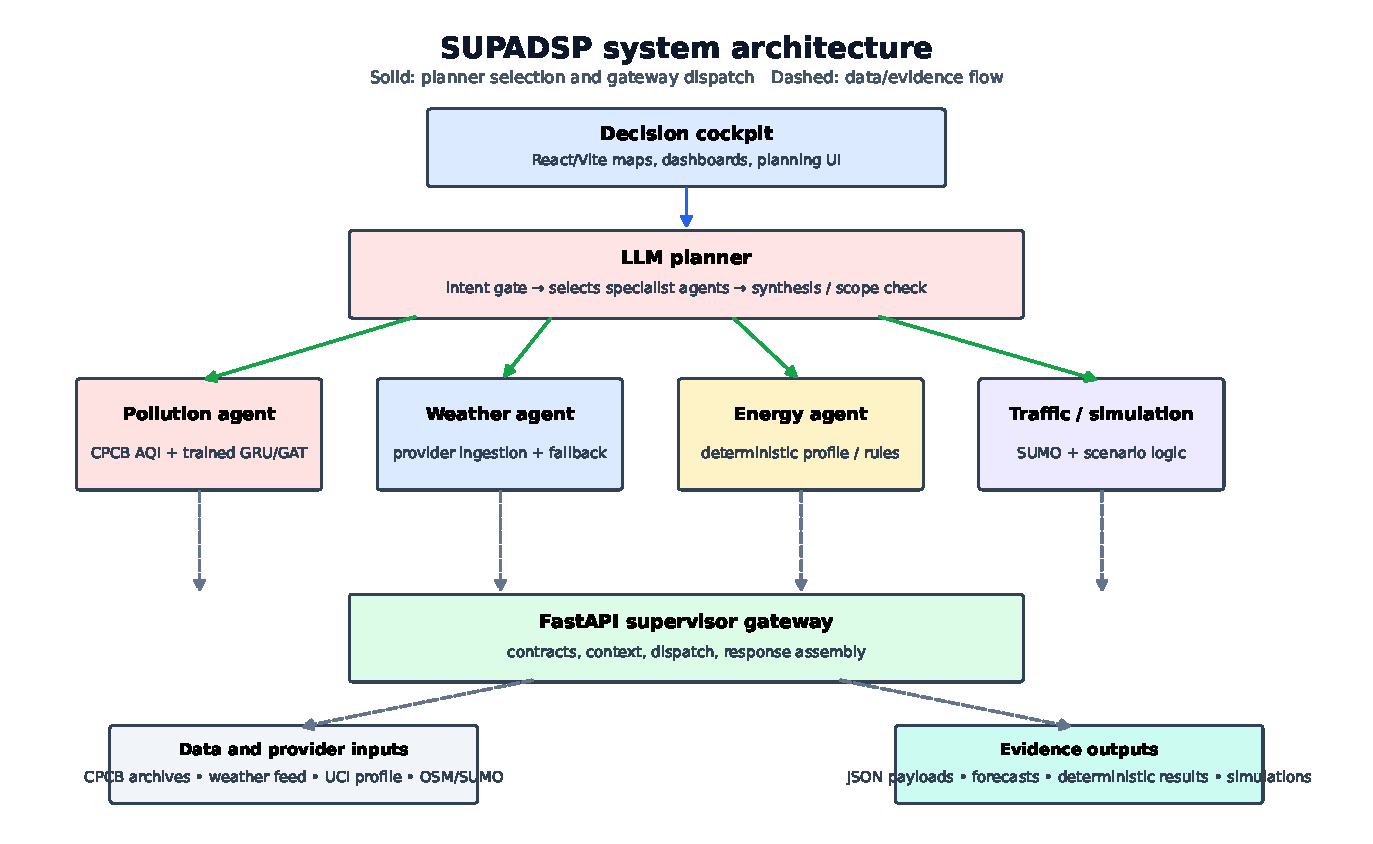
\includegraphics[width=0.96\textwidth]{figures/fig1_system_architecture.pdf}
\caption{SUPADSP architecture. Specialist agents return structured evidence to the supervisor and planner. The links to archived data, external provider responses, deterministic formulas, and SUMO are intentionally shown as different provenance paths.}
\label{fig:architecture}
\end{figure*}

Each contract describes purpose, required and optional inputs, output fields, provenance, freshness, and failure behavior. A response can therefore be useful without being treated as ground truth. For example, a traffic payload can state that it is a seeded simulation, while a pollution payload can identify the station and observation time. Missing data is represented as missing; the system does not replace it with a plausible number merely to complete a sentence.

\subsection{Three-stage planner}
Stage 1 interprets the query, gates out-of-scope requests, and selects capabilities. Stage 2 dispatches specialists, validates schemas, checks evidence sufficiency, and can request another dispatch when a required field is absent or contradictory. Stage 3 synthesizes a response and applies scope and numerical checks. The planner may return a bounded uncertainty statement instead of an estimate.

Let $q$ be a query, $C$ the capability set, and $E=\{e_i\}$ the returned evidence. The delivered response $r$ is accepted only when
\begin{equation}
 V(r,E)=V_{\rm scope}(r)\land V_{\rm numeric}(r,E)\land V_{\rm contract}(E).
\end{equation}
$V_{\rm numeric}$ checks that a number is present in evidence or is a declared derivation; it is not a proof that the underlying measurement is correct. $V_{\rm contract}$ checks the schema and capability boundary. The scope check removes internal markers and unrelated material. This formalization makes clear why grounding compliance is narrower than factual accuracy.

\subsection{Provenance model}
We use five provenance classes: (i) archived or observed data, (ii) external-provider data, (iii) learned estimates, (iv) deterministic or rule-based outputs, and (v) simulation outputs. A single response can contain several classes. The provenance label travels with a field rather than being inferred from prose. Figure~\ref{fig:provenance} depicts this separation.

\begin{figure*}[t]
\centering
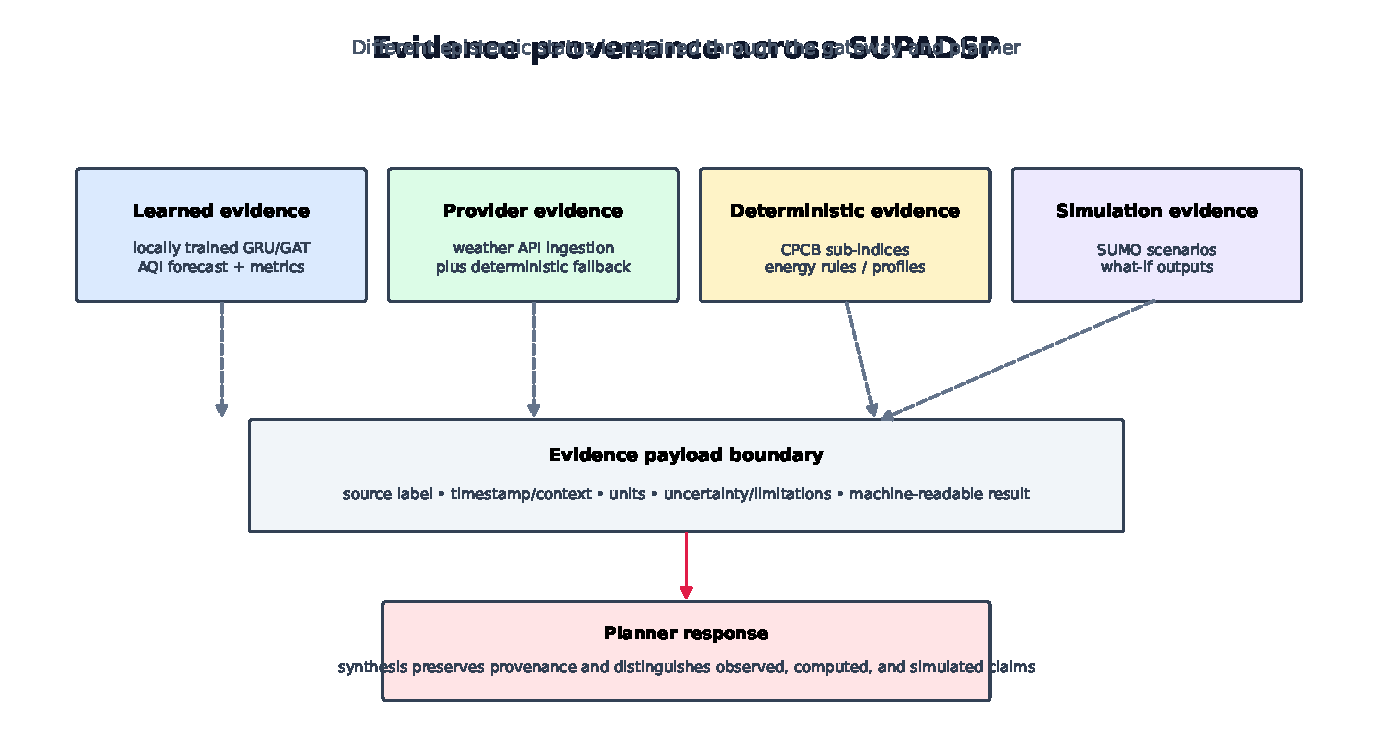
\includegraphics[width=0.96\textwidth]{figures/fig4_evidence_provenance.pdf}
\caption{Evidence provenance classes used by the platform. The planner may combine classes for a decision-support answer, but it preserves whether a value was observed, provider-derived, learned, deterministic, or simulated.}
\label{fig:provenance}
\end{figure*}

\subsection{Implementation status}
Table~\ref{tab:status} summarizes the implementation boundary. A ``yes'' means that the mechanism exists in the inspected source; it does not mean that an independent accuracy study exists.

\begin{table}[t]
\caption{Implementation and evidence status.}
\label{tab:status}
\centering\scriptsize
\begin{tabular}{@{}lccccc@{}}
\toprule
Component & Learned & Provider & Deterministic & Simulation & Evidence limit\\
\midrule
Pollution & yes & partial & yes & no & archive/test scope\\
Weather & no & yes & fallback & no & no local skill study\\
Energy & no & no & yes & no & household profile\\
Traffic & no & no & rules & yes & synthetic demand\\
Planner & no & model path & checks & no & finite artifacts\\
\bottomrule
\end{tabular}
\end{table}

\subsection{Failure semantics and user-visible states}
The platform distinguishes four states that are often collapsed in dashboard implementations. \emph{Available} means that a response satisfies its contract and has the expected provenance fields. \emph{Stale} means that a value exists but exceeds the freshness threshold configured for that source. \emph{Unavailable} means that the provider or specialist did not return a usable payload. \emph{Insufficient} means that a payload arrived but lacks the fields required for a domain computation, such as the minimum pollutant set for AQI. These states are carried to the planner instead of being converted to zeros.

This state model also limits cross-domain composition. A stale weather value may still be shown as context if its timestamp is visible, but it should not silently drive a fresh alert. A traffic simulation can be executed when live traffic data is absent, but the response must say that it is a scenario. A pollution forecast can be generated from the archive before the live switchover threshold is met, but its source is archive evidence rather than live telemetry. In this way, graceful degradation changes the claim made by the system instead of hiding degradation.

The same principle applies to transport errors. In-process execution reduces deployment complexity but does not make the specialist's numerical output more authoritative. HTTP execution introduces timeouts and serialization failures, so the supervisor records transport status separately from domain status. A successful HTTP response can still carry an insufficient AQI payload; conversely, a failed external call does not imply that a deterministic fallback is a measured substitute. These distinctions are especially important for a planner because language synthesis tends to smooth categorical differences unless they are represented explicitly in the input schema.

\section{Air-Quality Agent}
\label{sec:pollution}
\subsection{Data and feature construction}
The configuration declares 13 TSPCB CAAQMS stations and six forecast targets: PM$_{2.5}$, PM$_{10}$, NO$_2$, SO$_2$, CO, and O$_3$. The CPCB engine additionally accepts NH$_3$; lead is not implemented. The local feature vector has seven pollutant inputs (the six targets plus NH$_3$), five meteorological inputs (air temperature, relative humidity, wind speed, pressure, and solar radiation), and six cyclic temporal features. Thus the local dimensionality is $7+5+6=18$. The deployed spatial variant appends six inverse-distance-weighted covariates from neighboring stations; it is not an 18-feature model with an ambiguous spatial dimension.

For station $s$ at day $t$, the model consumes a 14-day context and predicts seven days, D1--D7. For each neighbor set $N_k(s)$ with $k=3$, a spatial covariate is formed as
\begin{equation}
 z_{s,t}=\frac{\sum_{j\in N_k(s)}d_{sj}^{-1}x_{j,t}}{\sum_{j\in N_k(s)}d_{sj}^{-1}},
\end{equation}
where distances are Haversine distances and $x_{j,t}$ is the corresponding neighbor feature. The source code also defines a distance-weighted graph variant; its comparison is an ablation, not evidence that any particular physical mechanism causes an error difference.

The archive-to-live mechanism requires 14 consecutive valid live days before switching the forecast input source. This is an operational guard, not a live-data accuracy validation. The present reported forecast metrics are tied to the recorded archive and evaluation artifacts; no claim is made that the model has been validated after that switch.

\subsection{CPCB computation}
For pollutant $p$ and concentration $C$, the sub-index is obtained by breakpoint interpolation:
\begin{equation}
 I_p=\frac{I_{hi}-I_{lo}}{C_{hi}-C_{lo}}(C-C_{lo})+I_{lo}.
\end{equation}
The reported AQI is the maximum available sub-index. The implementation requires at least three valid pollutants, including PM$_{2.5}$ or PM$_{10}$, and returns no AQI when the requirement is not met. This is a data sufficiency rule, not imputation.

The implementation cross-check contains 12 rows: 11 regional station rows and one NSIT Delhi reference row. It must not be described as a 13-station field validation or as a denominator of 13 local rows. Four rows match exactly and seven are within two AQI points, including the exact matches; the remaining five differ by more than two. The prominent pollutant agrees in the recorded rows. Differences are consistent with the implementation using calendar-day arithmetic means while the bulletin comparison uses a retrospective 24-hour window ending at a specified time. This comparison tests an implementation against published rows; it does not establish network-wide operational accuracy.

\subsection{Candidate predictors and selection record}
The candidate set contains a two-layer TemporalGRU\_KNNCovariate (hidden size 64, dropout 0.15), a temporal-only GRU, a distance-weighted GAT--GRU, Chronos-2 with covariates, persistence, and a seven-day seasonal naive baseline. Chronos-2 is an externally implemented foundation-model candidate; the paper does not attribute its behavior to a local retraining procedure.

The metadata records three seasonal rolling-origin validation folds: monsoon washout (train through 2024-06-30, validate July--September 2024), winter inversion peak (train through 2024-10-31, validate November 2024--January 2025), and summer transition (train through 2025-03-31, validate April--June 2025). The later test period is October--December 2025. These dates are reported as artifact metadata, not as a claim that the folds exhaust all possible seasonal regimes.

The model artifact identifies TemporalGRU\_KNNCovariate as the selected winner. During development, test metrics were exposed during the model lock-in discussion. Consequently, the later test numbers are descriptive evidence of generalization for the recorded artifact, not the result of a pristine blind test or a recommendation to choose a model by the test gap. The validation record remains the selection-facing record; the test record is reported with this contamination caveat.

\begin{figure*}[t]
\centering
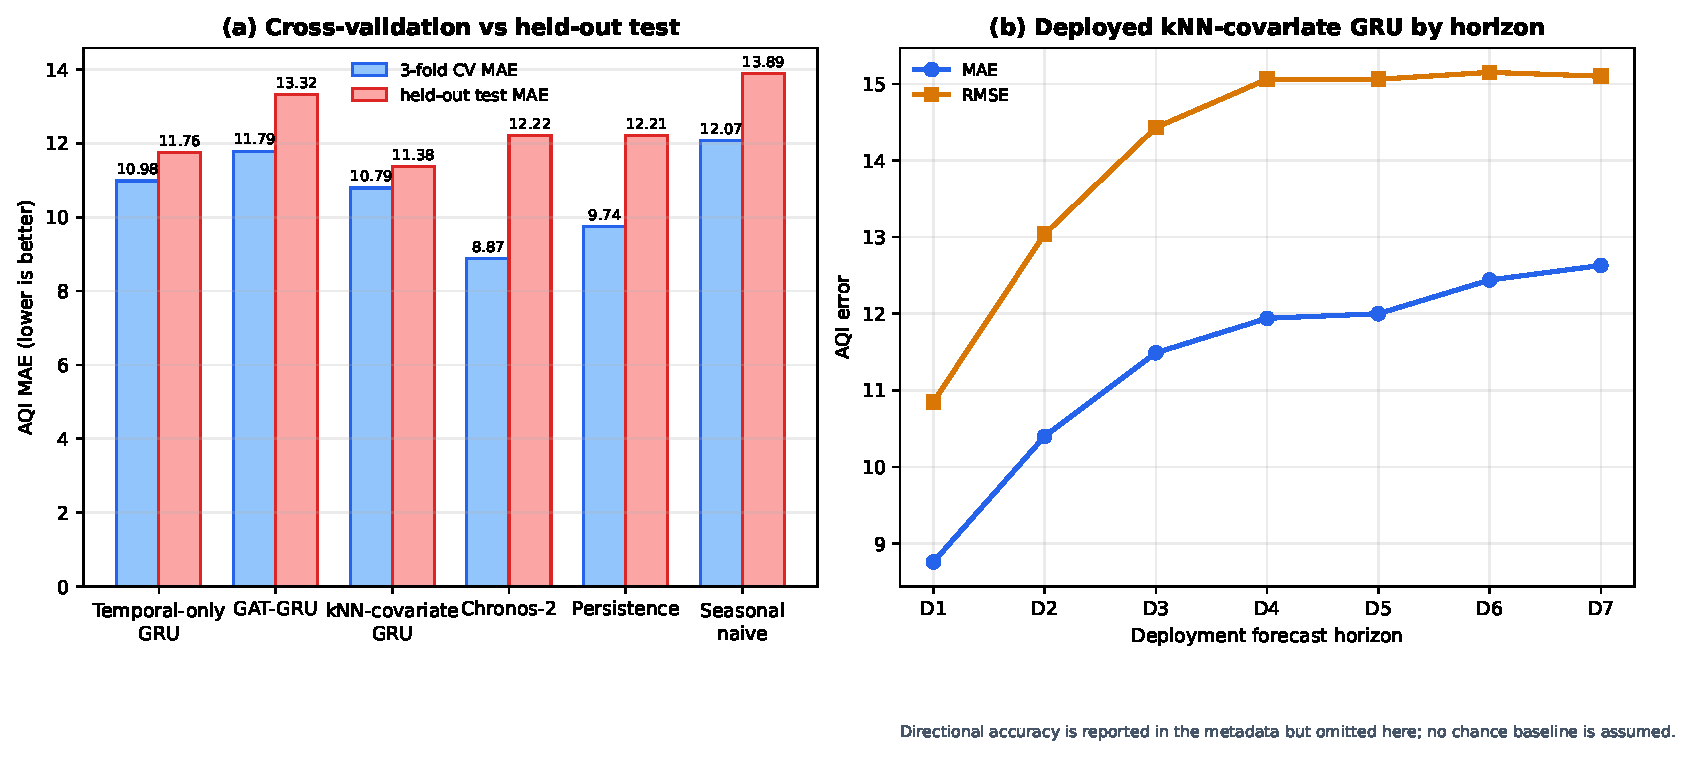
\includegraphics[width=0.96\textwidth]{figures/fig2_forecasting_evaluation.pdf}
\caption{Forecasting evaluation artifact: seasonal validation and later-period comparison, with model and horizon error plots. The figure is read together with the provenance note in Section~\ref{sec:pollution}; it does not convert an exposed test result into a blind selection result.}
\label{fig:forecast}
\end{figure*}

\section{Weather, Energy, Traffic, and Simulation}
\label{sec:otherdomains}
\subsection{Weather ingestion}
The weather agent is a FastAPI service with health and current-weather endpoints. When configured, it requests values from the external provider; otherwise it returns a static deterministic fallback. The service caches a response for a short interval. It does not train a weather model, and the repository does not provide an independent local station archive for MAE, RMSE, calibration, or alert-skill evaluation. We therefore use weather as contextual provider-derived evidence. No attribution to a particular numerical weather prediction model is made here, because the inspected application exposes provider fields rather than a verified upstream model record.

The platform contains cross-domain coefficients for rainfall, HVAC temperature response, pollutant dispersion labels, and similar scenario logic. They are engineering assumptions. They are not learned causal effects, and the paper does not interpret them as estimates of an intervention.

\subsection{Energy profile}
The energy agent combines an empirical hourly profile with a Gaussian diurnal curve:
\begin{equation}
 W(t)=0.85W_{\rm emp}(h)+0.15G(t),
\end{equation}
where $W_{\rm emp}$ is derived from the UCI household dataset and $G$ is a fixed multi-peak curve. Temperature, EV count, traffic occupancy, and solar capacity then modify generated scenario values through fixed coefficients. Substation names, capacities, and values are a registry and model output; they are not SCADA measurements.

The available evaluator reads 150,000 sampled household rows, uses the last 30\% as a chronological evaluation slice, and reports a rerun MAPE of 17.32\%, MAE 0.1988 kW, RMSE 0.2488 kW, and $R^2=0.8443$. However, the empirical hourly means used to form $W_{\rm emp}$ are computed before the split from all sampled rows. The profile therefore contains test-period information. We call the result a leakage-affected diurnal-profile fit, not an out-of-sample grid forecast. The reported 100\% top-eight overlap is a ranking overlap on the same diagnostic and is not a peak reliability guarantee.

\subsection{Traffic provenance and simulation}
The traffic service runs Eclipse SUMO scenarios~\cite{lopez2018microscopic} on the configured Narayanguda network. Its API defaults to a synthetic-normal scenario, a 120-simulation-second duration, and seed 42. The output contains scenario KPIs such as speed, delay, queues, throughput, and emissions estimates. These are simulation outputs.

The separate traffic-data generator is also synthetic: it defines 15 named intersections, creates 15-minute timestamps over 2023, uses seed 42, constructs demand from morning and evening Gaussian rush profiles, adds random noise, and derives speed, volume, occupancy, and congestion from capacities and free-flow speeds. The generated CSV is therefore useful for deterministic software tests and interface development, not a measured sensor dataset. We do not use its values as field evidence.

The planner may request a baseline scenario or validate signal parameters. A signal candidate is not an intervention study. Without repeated seeds, an independently specified policy baseline, and observed traffic measurements, a difference between two simulations cannot establish causal congestion reduction.

\begin{figure*}[t]
\centering
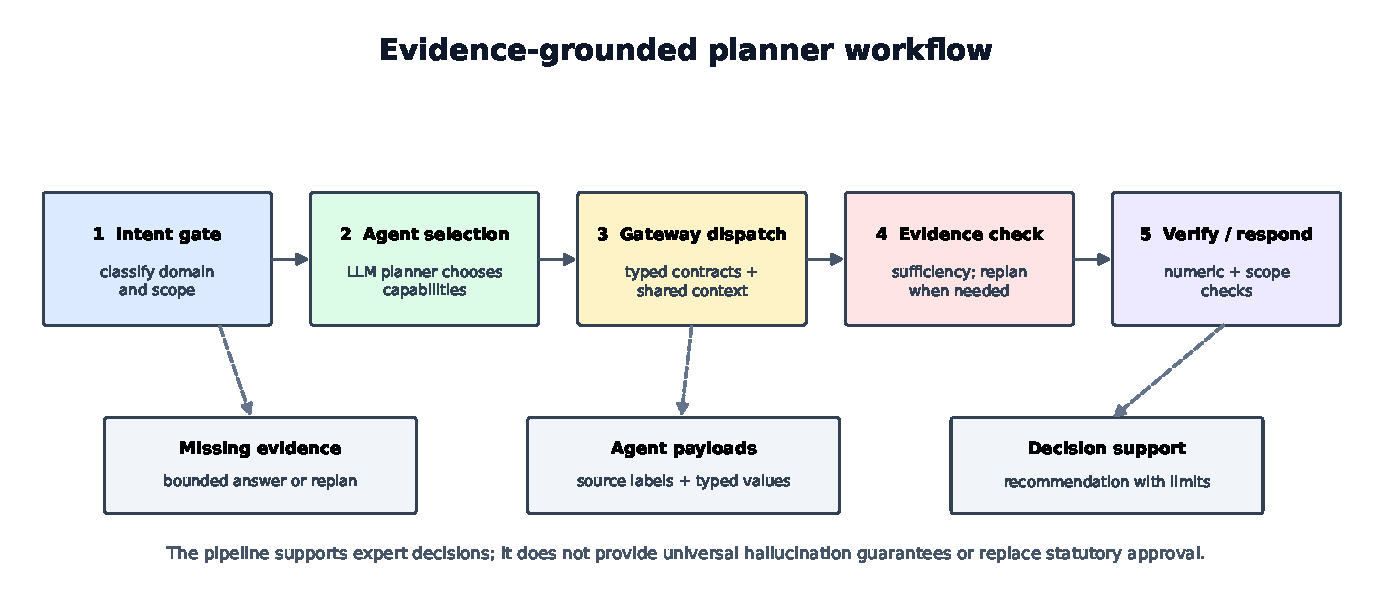
\includegraphics[width=0.96\textwidth]{figures/fig3_grounded_planner_workflow.pdf}
\caption{Grounded planner workflow. Query gating precedes specialist dispatch; evidence is checked before synthesis; final scope and numerical checks operate on the response artifact. The end-to-end and golden-set evaluation quantities are distinct and are reported separately.}
\label{fig:planner}
\end{figure*}

\section{Planner Evaluation}
\label{sec:planner}
The planner routes queries to pollution, weather, energy, traffic, simulation, or multi-domain capabilities. It exposes a rule-based fallback for selected advice paths and can return unavailable or stale states. Numeric verification is lexical and schema-aware: a number in a response must be supported by a payload or by a declared computation. This does not verify an external provider or a simulated world; it verifies that the response did not silently invent a number relative to its evidence.

The evaluation artifacts must be kept separate. The end-to-end planner artifact contains 81 passes out of 85 cases. A separate curated golden-set checker reports 123/123 grounding-compliance passes. The latter is not a substitute for the former, and neither is a claim of general factual accuracy. A non-pollution regression artifact reports 20/20; advice-mode artifacts report 15/15 on the available LLM-on subset and 60/60 on the rule-fallback and reasoning-false checks. These counts are finite, checker-defined outcomes. They do not establish robustness to arbitrary prompts, prompt injection, unseen provider failures, or changes in the underlying services.

\begin{figure}[t]
\centering
\begin{minipage}{0.95\columnwidth}
\footnotesize
\textbf{Algorithm 1: Evidence-bounded planner execution.}\\
\textbf{Input:} query $q$, contracts $C$.\\
1. Classify and gate $q$. If it is out of scope, return a bounded rejection.\\
2. Dispatch required capabilities under $C$ and collect $E$.\\
3. Check schema, freshness, and evidence sufficiency. Retry, re-dispatch, or mark unavailable when a check fails.\\
4. Synthesize response $r$ from $E$.\\
5. If $V_{\rm scope}(r)\land V_{\rm numeric}(r,E)\land V_{\rm contract}(E)$ holds, return $r$ with provenance; otherwise return a bounded evidence-status response.
\end{minipage}
\caption{IEEE-compatible figure float for the evidence-bounded planner procedure.}
\label{fig:algorithm}
\end{figure}

\section{Evaluation Protocol and Metrics}
\label{sec:metrics}
The central unit of analysis is declared before a number is interpreted. For scalar targets, MAE and RMSE are
\begin{equation}
 \mathrm{MAE}=\frac{1}{n}\sum_i|y_i-\hat y_i|,\qquad
 \mathrm{RMSE}=\sqrt{\frac{1}{n}\sum_i(y_i-\hat y_i)^2}.
\end{equation}
Category accuracy is the fraction of forecast AQI categories equal to the CPCB category of the target. Directional accuracy compares signs of successive changes in a horizon sequence; because the recorded implementation has no uncertainty calibration or established null distribution, values are reported descriptively. In particular, 50\% is not treated as an established chance result for this data and metric implementation.

For energy, MAPE is computed against hourly normalized-profile values after rescaling to the held-out slice mean. Because the predictor's hourly weights use all rows, leakage changes the interpretation. For traffic, counts and means are scenario measurements, not estimates of a population parameter. For planning, a pass is defined by the evaluator's checker; it is not an independently adjudicated factual-accuracy label.

\subsection{Evaluation units and aggregation}
The pollution evaluator receives arrays indexed by forecast origin, horizon, and target pollutant. It clips predicted concentrations at zero before computing pollutant and AQI measures. AQI is recomputed from the predicted concentrations using the same CPCB engine used for targets; consequently, a concentration error does not map linearly to an AQI error near a breakpoint. Overall AQI metrics flatten forecast origins and horizons, whereas the horizon table retains the horizon index. This distinction matters when comparing a seven-day aggregate with D1: the former weights all available horizons, while the latter uses only the first predicted day.

The metadata records per-fold metrics as means and standard deviations across three seasonal folds. These standard deviations describe fold-to-fold variation, not a confidence interval over independent cities or years. The evaluation does not bootstrap forecast origins, test multiple station holdouts, or correct for repeated comparisons. A future protocol should report station-level distributions, forecast-origin confidence intervals, and a pre-registered primary metric. It should also specify whether a city AQI is a maximum over stations, a station average, or another aggregation; the current artifact evaluates the city-shaped tensor produced by the unified evaluator and should not be generalized to an unspecified city aggregation.

\subsection{Operational checks versus accuracy checks}
The system has several checks that are valuable even when accuracy is unknown. Health endpoints test service availability. Contract checks test that required fields and types are present. Freshness metadata can identify stale external observations. Artifact guards test that a model class is compatible with its serializer. Numerical grounding checks test support in a returned payload. None of these checks measures forecast skill. Conversely, a low MAE does not prove that a response is safe to use if the response loses its source, time, or provenance label. We therefore report operational and statistical evidence in separate columns in Table~\ref{tab:summary}.

This distinction also explains why the planner can legitimately decline a query. If the weather provider is unavailable, returning a static fallback with its deterministic provenance is different from presenting that fallback as a forecast. If fewer than three pollutants are valid, the AQI engine returns no AQI rather than lowering the sufficiency rule. If a simulation contains no tracked vehicles, a missing KPI is different from zero speed or zero delay. These behaviors reduce silent substitution, but they can also reduce apparent completion rates. The end-to-end planner artifact should therefore be read together with its failure cases rather than as a standalone success percentage.

\section{Results}
\label{sec:results}
\subsection{Pollution validation and test records}
Table~\ref{tab:cv} reproduces the recorded three-fold validation summary. Chronos-2 has the lowest mean MAE in this artifact, while the selected TemporalGRU\_KNNCovariate has a higher mean and materially higher fold variability. The metadata also records the winter fold as difficult for all candidates. We do not infer a mechanism from these differences.

\begin{table}[t]
\caption{Recorded seasonal validation metrics (mean $\pm$ standard deviation).}
\label{tab:cv}
\centering\scriptsize
\begin{tabular}{@{}lrrr@{}}
\toprule
Model & AQI MAE & AQI RMSE & Cat. acc.\\
\midrule
Chronos-2 covariates & $8.87\pm0.23$ & $14.06\pm2.29$ & 79.9\%\\
Persistence & $9.74\pm0.30$ & $15.08\pm1.51$ & 80.7\%\\
TemporalGRU\_KNN & $10.79\pm3.74$ & $14.09\pm2.46$ & 69.4\%\\
Temporal-only GRU & $10.98\pm3.50$ & $14.37\pm2.04$ & 65.8\%\\
GAT--GRU weighted & $11.79\pm4.31$ & $15.13\pm2.95$ & 67.5\%\\
Seasonal naive & $12.07\pm1.01$ & $17.34\pm1.18$ & 73.5\%\\
\bottomrule
\end{tabular}
\end{table}

The later test record is shown in Table~\ref{tab:test}. TemporalGRU\_KNN has MAE 11.38, compared with 11.76 for the temporal-only GRU, 12.21 for persistence, 12.22 for Chronos-2 with covariates, 13.32 for GAT--GRU, and 13.89 for seasonal naive. The difference between KNN and temporal-only is 0.38 AQI points in this record. Since test results were visible during development, these values document observed behavior and cannot be used to claim blind generalization or to prescribe selecting by the test gap.

\begin{table}[t]
\caption{Recorded later-period AQI test metrics; test exposure limits the claim.}
\label{tab:test}
\centering\scriptsize
\begin{tabular}{@{}lrrr@{}}
\toprule
Model & MAE & RMSE & Cat. acc.\\
\midrule
TemporalGRU\_KNN & 11.38 & 14.18 & 63.95\%\\
Temporal-only GRU & 11.76 & 14.08 & 64.29\%\\
Persistence & 12.21 & 15.93 & 59.47\%\\
Chronos-2 covariates & 12.22 & 15.60 & 64.12\%\\
GAT--GRU weighted & 13.32 & 15.81 & 65.12\%\\
Seasonal naive & 13.89 & 17.91 & 61.46\%\\
\bottomrule
\end{tabular}
\end{table}

The per-horizon record for the selected model is: D1 MAE 8.76 and RMSE 10.85; D2 10.40 and 13.04; D3 11.49 and 14.43; D4 11.94 and 15.06; D5 12.00 and 15.06; D6 12.44 and 15.15; and D7 12.63 and 15.10. Directional values are 40.0\%, 36.5\%, 23.5\%, 36.5\%, 36.5\%, 45.9\%, and 42.4\%, respectively. These numbers show that level error and direction agreement are different properties; they do not establish that the model is below a formally defined chance baseline.

\subsection{CPCB and cross-domain records}
The CPCB cross-check has four exact matches and seven within $\pm2$ across 12 rows, with five greater divergences. The correct denominator is 11 regional rows plus one Delhi reference. For energy, the rerun values are retained only as a leakage-affected diagnostic: MAPE 17.32\%, MAE 0.1988 kW, RMSE 0.2488 kW, $R^2=0.8443$. No weather MAE or RMSE is reported. Traffic outputs are scenario-specific; the inspected service exposes seeded SUMO KPIs but no field validation or independent intervention evaluation.

\begin{table}[t]
\caption{Evidence-aware summary of available measurements.}
\label{tab:summary}
\centering\scriptsize
\begin{tabular}{@{}p{1.0cm}p{2.05cm}p{2.05cm}@{}}
\toprule
Domain & Artifact & Interpretation\\
\midrule
Air & AQI MAE 11.38; RMSE 14.18; 12-row CPCB check & archive/test record; implementation cross-check\\
Weather & provider or static fallback & no local forecast validation\\
Energy & MAPE 17.32\%; MAE 0.1988 kW & leakage-affected household profile fit\\
Traffic & seeded SUMO KPIs & synthetic scenario output\\
Planner & 81/85 end-to-end; 123/123 golden checker & distinct finite artifacts\\
\bottomrule
\end{tabular}
\end{table}

\subsection{Answers to the research questions}
\textbf{RQ1 (spatial covariates).} The recorded comparison supports a cautious positive result for the particular KNN construction: its later-period MAE is 0.38 AQI points lower than the temporal-only GRU. The result is modest, the test was exposed during development, and there is no station-held-out experiment. It therefore does not establish that spatial covariates generally improve forecasting. It does establish that the extra six covariates were not uniformly harmful in this artifact.

\textbf{RQ2 (robustness across candidate classes).} The validation and later-period records disagree in rank. Chronos-2 has the lowest recorded validation MAE but is nearly tied with persistence on the later test record, while the selected KNN model has a smaller observed change from validation mean to test score. Because of test exposure, this is an observation about the artifact rather than a blind robustness estimate. The graph model's weaker score is similarly an empirical comparison, not evidence that attention is intrinsically unsuitable or that a particular physical process caused the difference.

\textbf{RQ3 (grounded responses).} The available artifacts provide evidence that the contracts and checkers can pass 81 of 85 end-to-end cases, with separate 123/123 golden and 20/20 regression checker results. These results support the narrower claim that the implementation can enforce its stated checks on those cases. They do not measure open-world factuality, user benefit, or resistance to every adversarial prompt. The 60/60 fallback artifact further indicates that a bounded rule path can be exercised when the language-model route is unavailable, but it does not show that the rules cover all urban advice.

\textbf{RQ4 (heterogeneous evidence).} The architecture answers this design question through explicit provenance classes and contract fields. It can place a learned AQI estimate beside provider weather context and a simulated traffic scenario without declaring them equivalent. This is an architectural property demonstrated by payload structure and workflow, not a measured social or operational impact. A field deployment study would need to test whether users actually preserve these distinctions when making decisions.

\subsection{Interpretation of negative evidence}
Negative results are useful only when the measurement boundary is clear. The GAT--GRU result is negative relative to the KNN and temporal baselines for the recorded later period, but it does not identify a causal reason. The direction values are low, but without a pre-specified null and uncertainty analysis they should not be labeled a statistically established chance failure. The energy score is numerically favorable on some measures, but leakage means it is not clean evidence of generalization. The planner's perfect golden-set checker result is encouraging, but the 81/85 end-to-end result shows why a single headline percentage would be misleading.

These distinctions also protect against an aggregation error in multi-domain papers. A platform can have a high response-compliance rate while its weather source has no local validation. It can have a lower AQI MAE than persistence while its forecast direction is unproven. It can produce plausible substation cards while using a household-scale profile. Reporting each evidence boundary is therefore part of the method, not merely a limitation section.

\section{Deployment-Governance Case Study}
\label{sec:governance}
The repository records a model-artifact identity failure. A deployment path assumed every candidate was a PyTorch module. When a non-PyTorch candidate reached serialization, an old fallback branch could save a temporal-only checkpoint under the selected candidate's label. The risk was not that one model had a particular score; it was that the artifact identity and the reported selection could diverge.

The remediation raises an error for unsupported model types, stages candidate artifacts, requires an explicit approval flag before promotion, and records the class and metrics in an audit record. This is consistent with the broader warning about hidden technical debt in machine-learning systems~\cite{sculley2015debt}. It is a governance control, not a claim that the full pipeline is formally verified. A future release should additionally bind model class, feature schema, training window, and checksum in one immutable manifest.

\section{Discussion}
\subsection{What the forecasting result means}
The recorded numbers support a narrow conclusion: under the available archive, splits, and implementation, the selected KNN-covariate GRU had a modestly lower later-period AQI MAE than the temporal-only ablation and persistence baseline, while graph attention and Chronos-2 were not better on that later record. The validation ranking was different. This is a useful warning about regime transfer, but it is not a universal ranking of architectures. Test exposure, a single station network, limited temporal coverage, and absent confidence intervals all constrain interpretation.

The model's direction scores should not be narrated as a discovered physical failure or as a statistically established below-chance effect. They indicate that the recorded level forecasts do not provide demonstrated directional skill under the implementation's sign comparison. A stronger study would pre-register a direction definition, specify treatment of zero changes, establish a null model, and report uncertainty over forecast origins.

\subsection{Why provenance matters}
A planner can be useful while combining evidence classes, provided the combination remains visible. A provider weather value can contextualize a rule-based energy estimate; a SUMO queue can support a scenario discussion; an AQI forecast can support a bounded risk statement. None of these combinations turns one class into another. The provenance graph in Fig.~\ref{fig:provenance} is therefore an interface requirement: a downstream user should be able to ask which source and transformation produced each number.

\subsection{Operational value and cost}
Contracts, freshness checks, and fallbacks make failures legible. Their cost is that the system returns ``unknown'' more often than a free-form assistant and that a checker can validate support without validating reality. Deterministic components are inspectable but depend on coefficients that require calibration. Learned components can absorb nonlinear patterns but require temporal evaluation and artifact identity controls. Simulation can test software and scenario sensitivity but cannot stand in for deployment measurement.

\section{Limitations and Threats to Validity}
\begin{enumerate}
\item \textbf{No blind test claim.} Test metrics were exposed during development. The later period is reported descriptively, and selection should not be justified by its gap.
\item \textbf{Archive and geography.} Pollution results cover one monitoring network and historical periods. Transfer to another city, network, emission mix, or climate is untested.
\item \textbf{Limited forecast evidence.} The test period contains 92 calendar days and rolling multi-day windows, but no confidence intervals, repeated seeds, or independent future release are supplied here.
\item \textbf{Feature and target limits.} Six pollutants are forecast; the CPCB engine supports seven criteria pollutants because lead is absent and NH$_3$ is used only by the AQI engine. Missingness and averaging choices can change AQI.
\item \textbf{CPCB comparison denominator.} The cross-check is 11 regional rows plus one Delhi reference, not all 13 local stations. Its averaging window is not identical to the bulletin window.
\item \textbf{Weather validation gap.} No independent local observation archive, calibration study, or verified upstream model attribution is included.
\item \textbf{Energy leakage.} The 17.32\% MAPE rerun uses hourly weights calculated from all sampled rows, including the evaluation slice. It is not a clean out-of-sample result, and household kW values do not validate substation MW behavior.
\item \textbf{Synthetic traffic.} The generated sensor data and SUMO demand are scenario artifacts. No claim of actual government deployment, field accuracy, or causal signal benefit is made.
\item \textbf{Planner artifacts.} The 81/85 end-to-end result and the separate 123/123 golden checker result have different denominators and should not be merged. Both are finite tests rather than universal factuality estimates.
\item \textbf{Provider and prompt risks.} External service outages, stale values, malicious tool payloads, schema drift, and prompt injection remain possible. Contracts reduce, but do not eliminate, these risks.
\end{enumerate}

\section{Conclusion and Future Work}
SUPADSP demonstrates a practical pattern for cross-domain urban decision support: specialist services can be coordinated without erasing whether a value is observed, provider-derived, learned, deterministic, or simulated. The pollution artifacts show why seasonal evaluation and simple baselines matter. The planner artifacts show measurable grounding compliance, but their denominators must remain explicit. The energy rerun and the absent weather validation show that a complete interface is not the same as a complete empirical study.

Future work should first create a genuinely untouched prospective pollution test and preregister model selection. It should recompute energy weights using training data only, then validate against local SCADA at an appropriate scale. Weather requires station-level observations and calibration metrics. Traffic requires measured counts, repeated seeds, a pre-specified policy comparison, and uncertainty intervals before any intervention claim. Planner evaluation should expand beyond curated cases with independent adjudication, adversarial payloads, and versioned provider fixtures. Finally, immutable manifests should bind model class, feature dimensions, data windows, provenance, and checksums so that an approved artifact is the artifact that runs.

\appendices
\section{Reproducibility Specification}
The inspected repository layout places specialists under \texttt{backend/agents/}, the supervisor under \texttt{backend/supervisor/}, evaluation artifacts under \texttt{eval/}, tests under \texttt{tests/}, and utility commands under \texttt{scripts/}. The forecasting metadata file is \texttt{backend/agents/pollution\_agent/unified\_forecast/artifacts/unified\_best\_model\_meta.json}; the feature and split declarations are in the corresponding \texttt{config.py}. The recorded seed is 42, batch size is 16, learning rate is $10^{-3}$, maximum epochs is 80, and early-stopping patience is 15. These settings specify the inspected artifact; they do not guarantee that a future rerun has identical library or provider versions.

The pollution context is 14 days and the horizon is seven days. The local feature dimension is 18, and the KNN variant adds six spatial covariates. The station count is 13. The archived training declaration begins 2024-01-01 and ends 2025-06-30; the later test declaration is 2025-10-01 through 2025-12-31. The seasonal metadata folds are listed in Section~\ref{sec:pollution}. The energy evaluator reads the first 150,000 rows available to its command, creates a 70/30 chronological split, and computes the empirical hourly profile before that split; this last fact is essential to reproducing the limitation.

\section{Metric and Evidence Definitions}
An \emph{observation} is a value present in an archived or measured source with a source identifier and time. A \emph{provider value} is returned by an external service and is not locally validated merely because it is structured. A \emph{learned estimate} is generated by a fitted model. A \emph{deterministic output} is calculated from declared formulas and coefficients. A \emph{simulation output} is produced by a specified scenario, seed, and simulator. A planner response can cite several classes, but the class of each field should be retained.

AQI MAE and RMSE operate on computed AQI values over forecast windows; pollutant MAE operates on concentration values and should not be compared numerically with AQI MAE. Category accuracy compares CPCB labels. MAPE is retained for the energy diagnostic because it is part of the evaluator, although percentage error can be unstable for small values. Peak overlap is the intersection of two sets of eight hourly indices divided by eight; it is not event detection precision or recall. A grounding pass means that the checker found required support and scope behavior for that case.

\bibliographystyle{IEEEtran}
\bibliography{references}
\end{document}
